\documentclass[UTF8]{ctexart}

\usepackage{amsmath}
\usepackage{float}
\usepackage{cases}
\usepackage{cite}
\usepackage{graphicx}
\usepackage[margin=1in]{geometry}
\geometry{a4paper}
\usepackage{fancyhdr}
\usepackage{booktabs}
\pagestyle{fancy}
\fancyhf{}


\title{两种测定蛋白质含量方法的实验比较}
\author{522111910161 尚子翔}
\date{\today}
\pagenumbering{arabic}

\begin{document}

\fancyhead[L]{}
\fancyhead[C]{两种测定蛋白质含量方法的实验比较}
\fancyfoot[C]{\thepage}

\maketitle
\tableofcontents
\newpage

\section{实验目的}
\begin{enumerate}
    \item 了解用双缩脲法测定蛋白质的原理和方法
    \item 了解用紫外线吸收法测定蛋白质含量的原理
    \item 比较两种蛋白质测定方法的优缺点
\end{enumerate}



\section{实验原理}
\begin{enumerate}
    \item Biuret Method(双缩脲法)

    
    Biuret can react with copper cation(铜离子)to give fuchsia(紫红色)complex in basic(碱性)solution. There are many peptide bonds in protein, their structure is familiar with biuret, so they also can give biuret reaction. Biuret can react with copper cation (铜离子)to give fuchsia(紫红色)complex in basic(碱性)solution.

\begin{figure}[H]
  \centering
  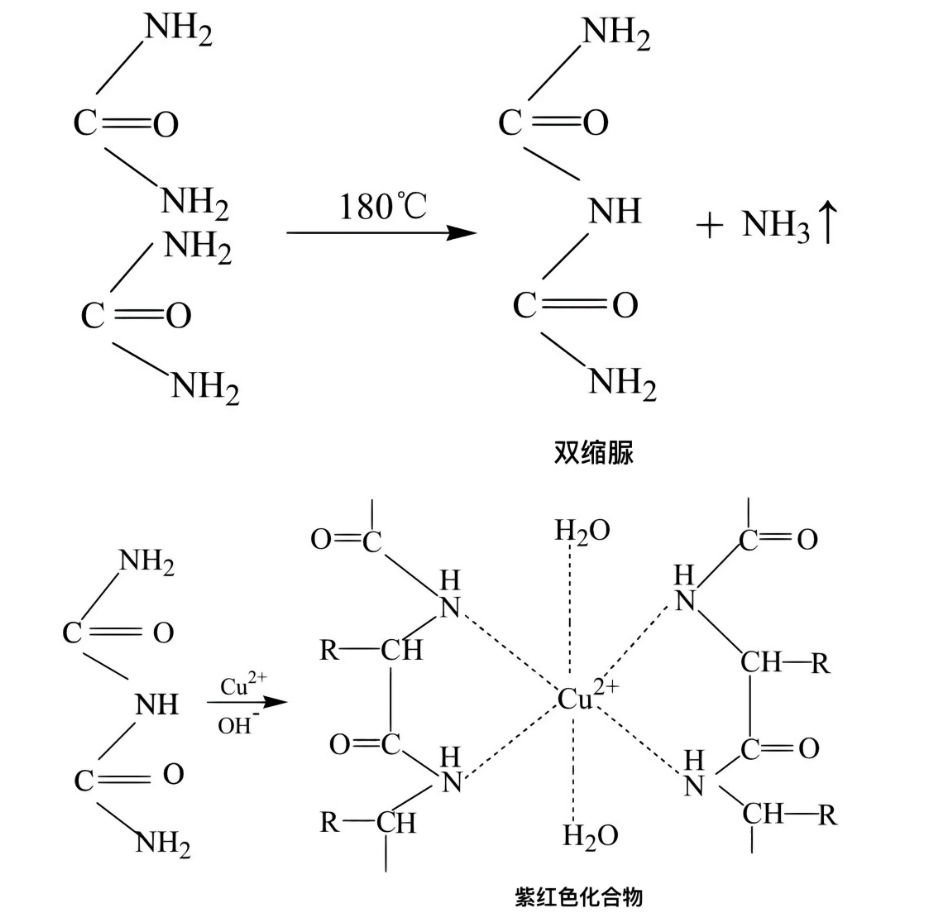
\includegraphics[scale = 0.5]{1.png} % 图片文件的名称和路径
  \caption{双缩脲试剂反应原理}
  \label{fig:example}
\end{figure}

    \item UV Absorption Method(紫外吸收法)
    
    Benzene rings of tyrosine and tryptophan residues contained in protein molecule have conjugated(共轭)double bonds which enable the protein to have maximum absorption value at the wavelength of 280 nm.
\end{enumerate}

\section{实验原理}

\subsection{试剂和设备}
\begin{itemize}
    \item 双缩脲试剂(Biuret reagent)
    \item 10 毫克/毫升标准蛋白质溶液
    \item 1 毫克/毫升标准蛋白质溶液
    \item 人血清(10、100 倍稀释)
\end{itemize}

\subsection{实验步骤与操作}
\subsubsection{双缩脲法}
\begin{enumerate}
    \item 制作标准曲线 \\
    取7支试管,按下表向试管中加入相应试剂,充分混匀后,室温下放置30min,测定$A_{540}$并以$A_{540}$为纵坐标,蛋白质浓度为横坐标,绘制标准曲线 \\
    \begin{table}[H]
        \centering
        \caption{双缩脲法测定蛋白质含量的试剂配置表}
        \begin{tabular}{cccccccc}
        \toprule
        & \multicolumn{6}{c}{试管编号} \\
        \cmidrule{2-7} 
        & 0 & 1 & 2 & 3 & 4 & 5 & 样品 \\
        \midrule
        10mg/mL 标准蛋白质溶液(mL) & 0.0 & 0.2 & 0.4 & 0.6 & 0.8 & 1.0 & 10倍稀释人血清 0.5 \\
        蒸馏水(mL) & 1.0 & 0.8 & 0.6 & 0.4 & 0.2 & 0.0 & 0.5 \\
        双缩脲试剂(mL) & 4.0 & 4.0 & 4.0 & 4.0 & 4.0 & 4.0 & 4.0\\
        \bottomrule
        \end{tabular}
    \end{table}
    \item 样品测定
    
  从标准曲线上查出待测蛋白质的浓度

    \item 数据计算
    
    样品蛋白质含量(mg/100mL)$=\frac{100cN}{v}$,其中c(mg/mL)为标准曲线查得的蛋白质浓度,N为稀释倍数,V为血清体积
    
\end{enumerate}

\subsubsection{紫外吸收测定法}
\begin{enumerate}
    \item 制作标准曲线

    取9支试管编号,按下表分别向每支试管加人各种试剂,摇匀。选用光程为1 cm 的石英比色杯,在280 nm 波长处分别测定各管溶液的$A_{280}$值。以$A_{280}$值为纵坐标,蛋白质浓度为横坐标,绘制标准曲线。
    \begin{table}[H]
        \centering
        \caption{紫外吸收法测定蛋白质含量的试剂配置表}
        \begin{tabular}{cccccccccc}
        \toprule
        & \multicolumn{8}{c}{试管编号} \\
        \cmidrule{2-9} 
        & 0 & 1 & 2 & 3 & 4 & 5 & 6 & 7 & 样品 \\
        \midrule
        1mg/mL 标准蛋白质溶液(mL) & 0.0 & 0.5 & 1.0 & 1.5 & 2.0 & 2.5 & 3.0 & 4.0 & 100倍稀释人血清 1.0 \\
        蒸馏水(mL) & 4.0 & 3.5 & 3 & 2.5 & 2.0 & 1.5 & 1.0 & 0.0 & 3.0 \\
        \bottomrule
        \end{tabular}
    \end{table}
    
    \item 样品测定

    从标准曲线上查出待测蛋白质的浓度

    \item 数据计算
    
    样品蛋白质含量(mg/100mL)$=\frac{100cN}{v}$,其中c(mg/mL)为标准曲线查得的蛋白质浓度,N为稀释倍数,V为血清体积
\end{enumerate}

\subsubsection{注意事项}
\begin{enumerate}
    \item 样品布需充分混匀,使用封口膜封住试管并且颠倒混匀
    \item 确保试管洁净
    \item 区分石英比色皿和玻璃比色皿,玻璃比色皿进能在540nm下使用
    \item 注意比色皿的光面和毛面,光面朝向光路
    \item 设置空白对照组,测定浓度由低至高,测定样品前需要用蒸馏水润洗比色皿
    \item 承装液体在$\frac{2}{3}$到$\frac{3}{4}$之间,如果比色皿光面站上液体需要擦拭干净
\end{enumerate}
\vfill
\section{实验数据记录和处理}

\subsection{双缩脲法}


\begin{table}[H]
    \centering
    \caption{紫外吸收法测定蛋白质含量的数据记录表}
    \begin{tabular}{cccccccc}
    \toprule
    & \multicolumn{6}{c}{试管编号} \\
    \cmidrule{2-7} 
    & 0 & 1 & 2 & 3 & 4 & 5 & 样品 \\
    \midrule
    10mg/mL 标准蛋白质溶液(mL) & 0.0 & 0.2 & 0.4 & 0.6 & 0.8 & 1.0 & 10倍稀释人血清 0.5 \\
    蒸馏水(mL) & 1.0 & 0.8 & 0.6 & 0.4 & 0.2 & 0.0 & 0.5 \\
    双缩脲试剂(mL) & 4.0 & 4.0 & 4.0 & 4.0 & 4.0 & 4.0 & 4.0\\
    A540 & 0.000 & 0.100 & 0.187 & 0.295 & 0.428 & 0.536 & 0.225 \\
    \bottomrule
    \end{tabular}
\end{table}



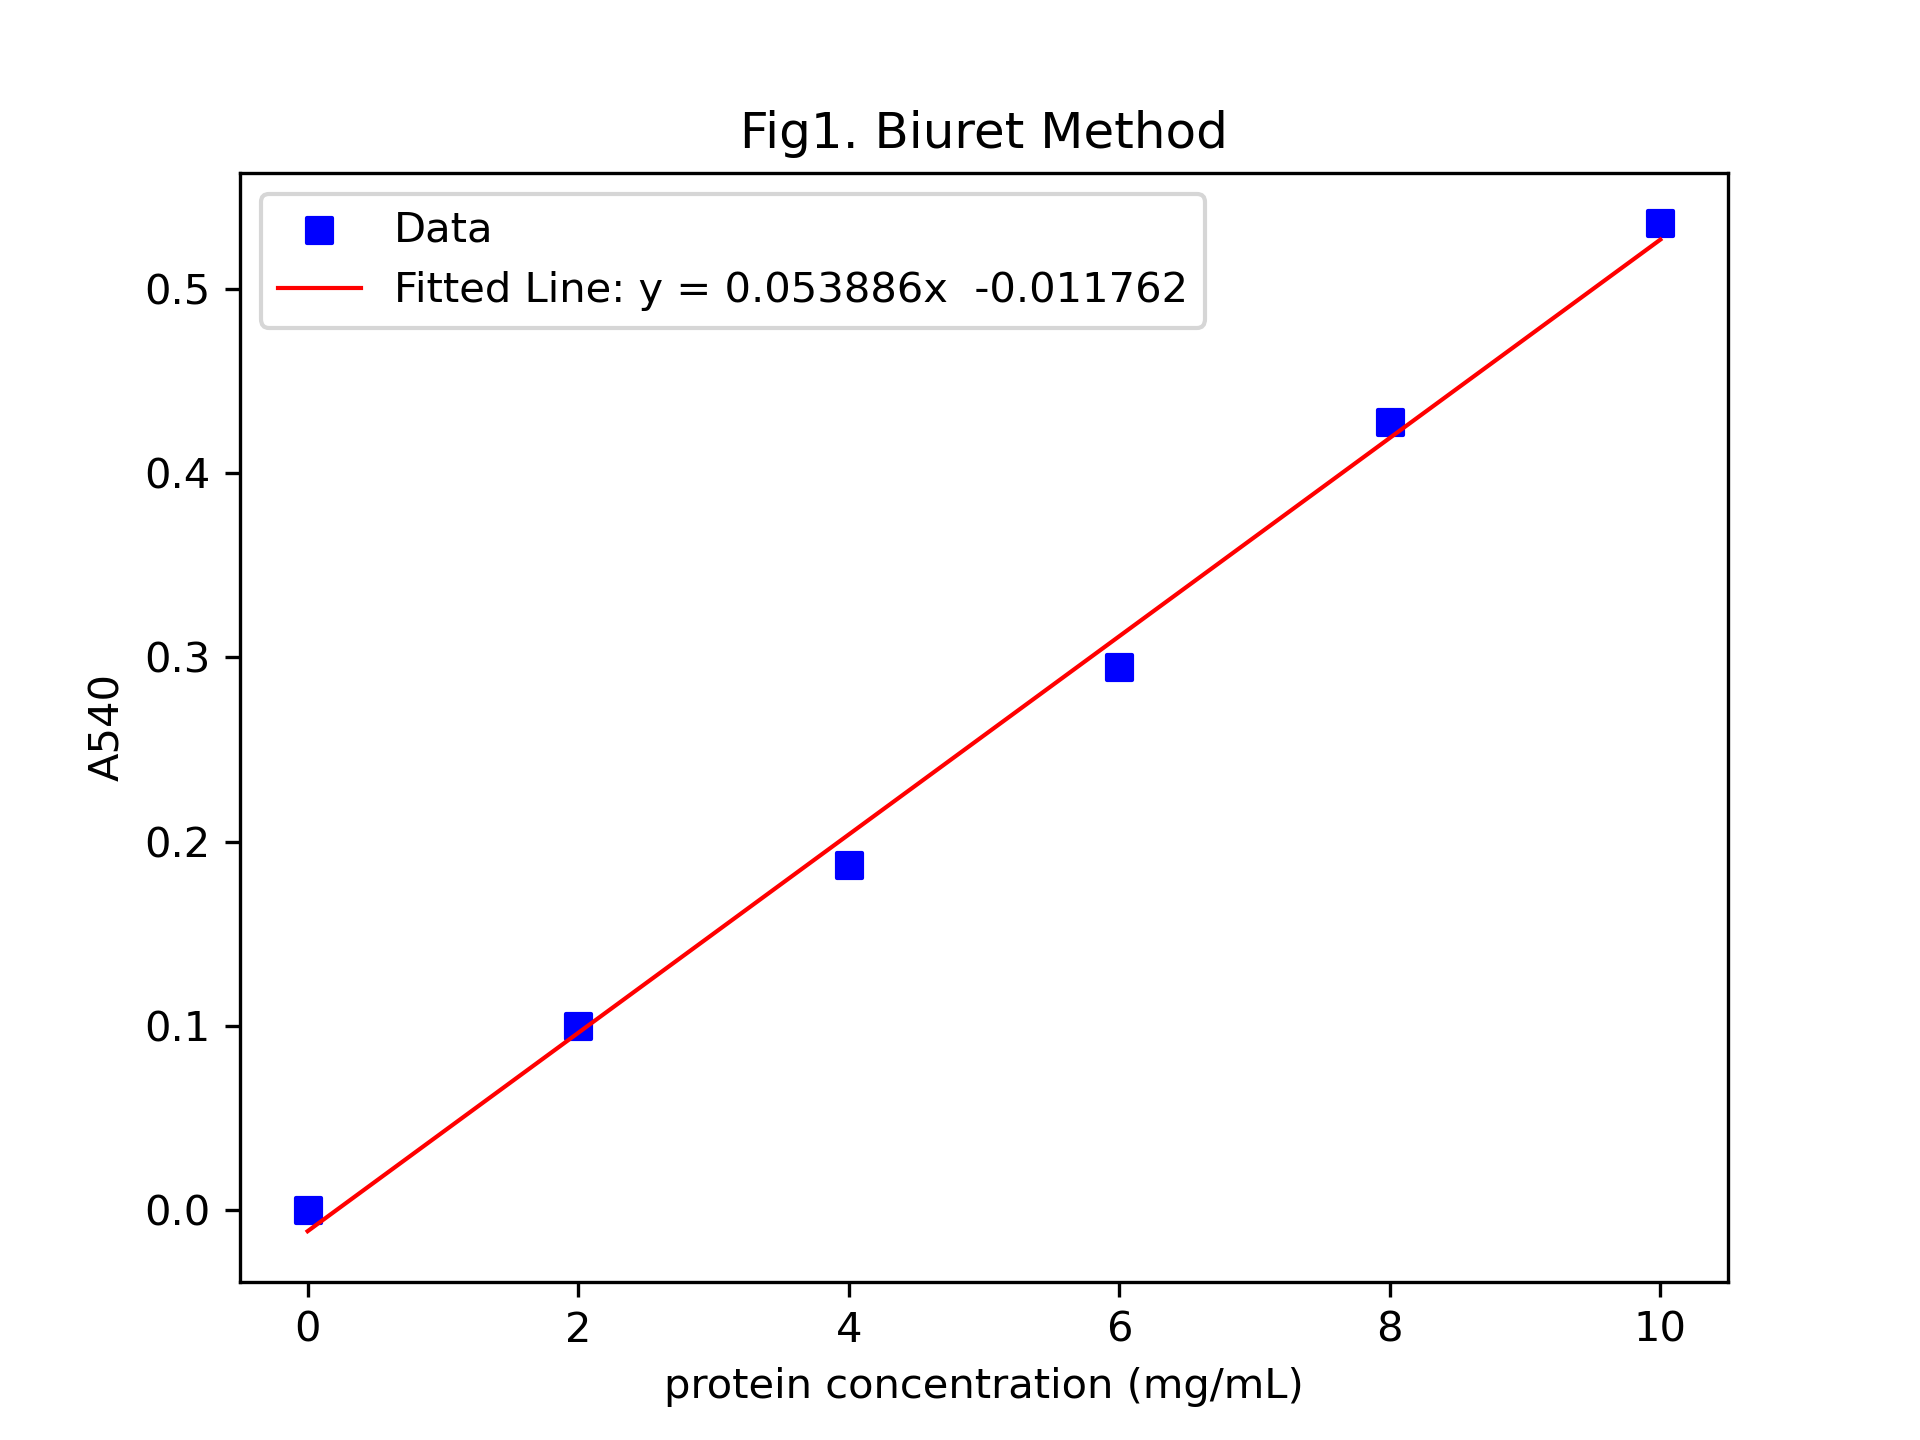
\includegraphics{A540.png}

\noindent{标准曲线:$y = 0.053886x-0.011762$ \\}
样品$A540=0.225$代入标准曲线计算得到蛋白质浓度为$4.393779mg/mL$\\
样品的蛋白质含量(mg/100mL)=$4.393779\times 10 \div 0.5 \times 100 =8787.5574mg/100mL$
\subsection{紫外吸收测定法}
\begin{table}[H]
        \centering
        \caption{紫外吸收法测定蛋白质含量的试剂配置表}
        \begin{tabular}{cccccccccc}
        \toprule
        & \multicolumn{8}{c}{试管编号} \\
        \cmidrule{2-9} 
        & 0 & 1 & 2 & 3 & 4 & 5 & 6 & 7 & 样品 \\
        \midrule
        1mg/mL 标准蛋白质溶液(mL) & 0.0 & 0.5 & 1.0 & 1.5 & 2.0 & 2.5 & 3.0 & 4.0 & 100倍稀释人血清 1.0 \\
        蒸馏水(mL) & 4.0 & 3.5 & 3 & 2.5 & 2.0 & 1.5 & 1.0 & 0.0 & 3.0 \\
		A280 & 0 & 0.097 & 0.161 & 0.252 & 0.347 & 0.434 & 0.534 & 0.696 & 0.204\\
        \bottomrule
        \end{tabular}
\end{table}

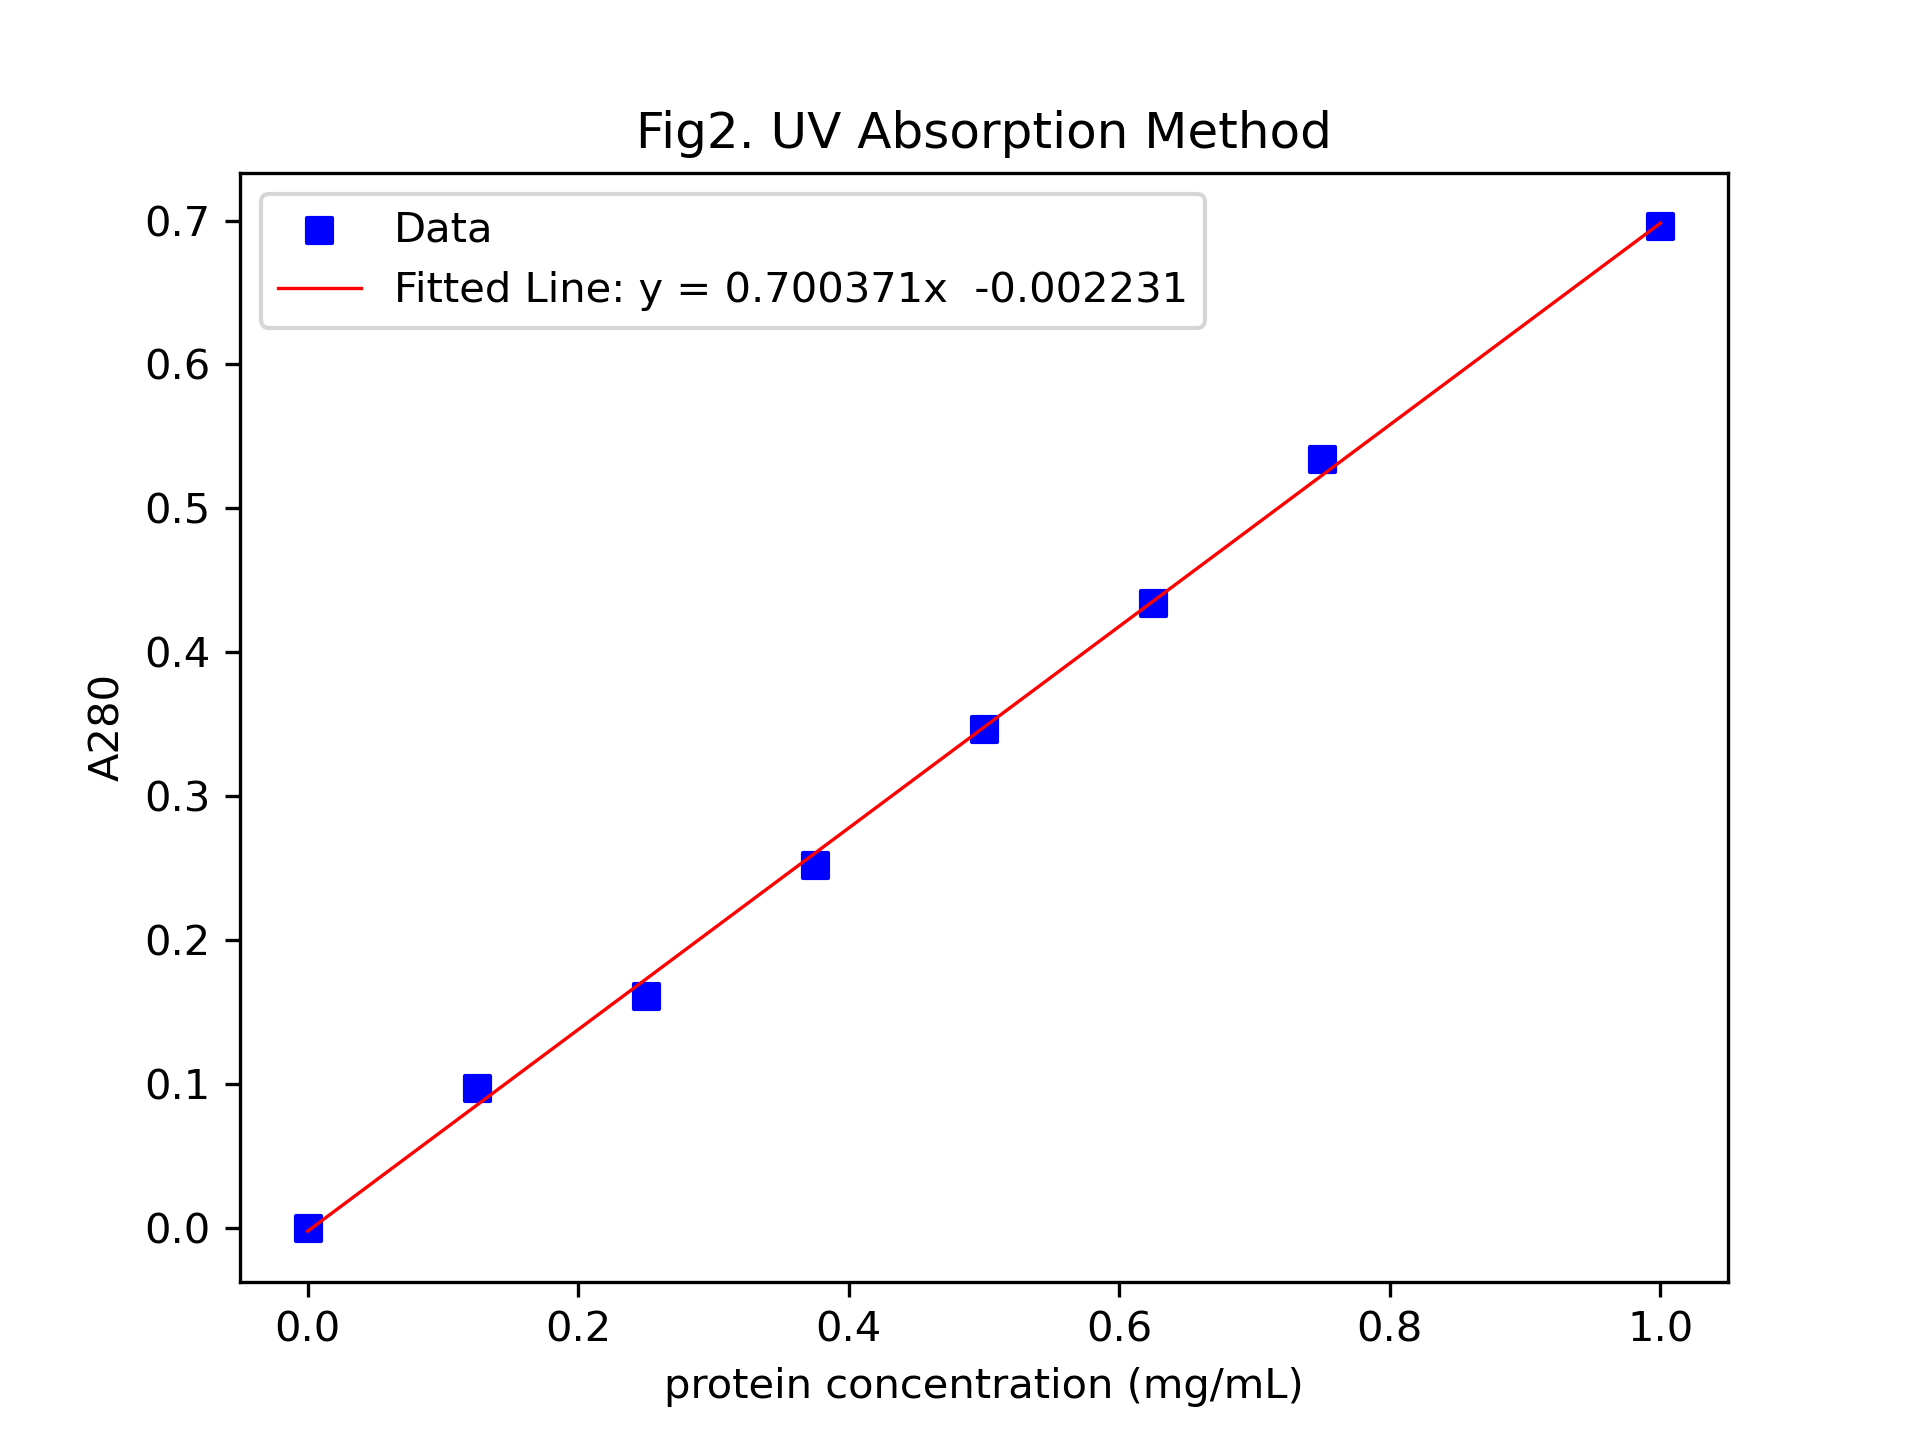
\includegraphics{A280.png}

\noindent{标准曲线:$y = 0.700371x-0.002231$ \\}
样品$A540=0.204$代入标准曲线计算得到蛋白质浓度为$0.294459mg/mL$\\
样品的蛋白质含量(mg/100mL)=$4.393779\times 100 \times 100 \times 4 =11778.3631mg/100mL$
\vfill
\section{实验结果分析讨论以及总结建议}
\subsection{实验结果分析讨论}

查阅相关资料得知人类血清中中蛋白含量大约为60-85mg/mL,推测本次实验中双缩脲测定方法比紫外吸光测定法准确,紫外吸光法测定的含量偏大。我认为可能的原因有以下几点:
\begin{enumerate}
    \item 操作不规范(例如测定样品前没有使用蒸馏水充分冲洗比色皿,导致样品的吸光度测定偏高)产生误差
    \item 样品中含有核酸类吸收紫外光的物质,使280nm处受到较大干扰,使紫外吸光测定法得到的结果偏高
    \item 双缩脲试剂不够灵敏,未充分混匀放置,导致双缩脲法测定的含量偏低
\end{enumerate}

\subsection{总结建议}
首先,我认为两种方法使用的情景不同:双缩脲操作简单,不需要昂贵的设备,但是不适合精度要求很高的实验,适合浓度较高的蛋白质样本,同时也需要去等待反应完全;紫外吸收法利用了含有共轭结构的氨基酸残基(酪氨酸、色氨酸、苯丙氨酸)在280nm处的光吸收定量测试,快捷方便,但是会受到核酸的干扰。

对于本实验的改进建议,我认为在使用紫外吸光法时,需要预先处理样品,使用酶处理或者是柱层析法将蛋白质与核酸分离提高精度;由于核酸在260nm处吸收紫外光,通过测定样品在280nm处和260nm处的紫外光吸收比例可以对于样品中蛋白质和核酸物质比有一定估计,从而矫正标准曲线得到更加准确的蛋白质含量

\section{思考题}
\subsection{干扰双缩脲实验的因素有哪些?}
\begin{itemize}
	\item 某些酸性或者碱性物质可能会影响蛋白质与双缩脲的反应
	\item 其他干扰反应的物质,例如:硫酸铵和Tris缓冲液
	\item 显色物质和胶体物质会影响样品的吸光度
\end{itemize}

\subsection{紫外吸收法若样品中含有核酸类杂质,应该如何矫正实验结果}
\begin{itemize}
	\item 利用酶处理或者柱层析的方法分离蛋白质和核酸类杂质
	\item 通过测量蛋白质样品在280nm和260nm处的吸光度,计算校正因子F
	\item 利用经验公式蛋白质浓度(mg/mL)=$1.45 \times A_{280}-0.74 \times A_{260}$
\end{itemize}
\end{document}




